\chapter{Literature Review}
\textbf{This chapter reviews the existing literature on autonomous mobile recognition systems, with a focus on sensor technologies, marker based localization, and robot control strategies. It analyzes the advantages and limitations of current methodologies to establish the theoretical framework for the proposed low-cost navigation system. Additionally, the Preferred Reporting Items for Systematic Reviews and Meta-Analysis (PRISMA) guidelines was done to ensure a systematic and transparent process of searching, screening, and inclusion of literature.}
\section{Search Strategy}
\index{Search Strategy|(}
To begin the literature review process and identify relevant studies, the researchers conducted a literature search across Google Scholar, IEEE Xplore, and arXiv. The search was done specifically with the query strings shown in Table 2.1 below. Query strings were varied for each database to ensure that the strings were syntactically correct with each database’s unique search syntax.

\begin{table}[htbp]
\centering
\setlength{\tabcolsep}{4pt}
\begin{tabular}{>{\raggedright\arraybackslash}p{3cm}
                >{\raggedright\arraybackslash}p{11cm}}
\hline
\textbf{DATABASE} & \textbf{Query String} \\
\hline
Google Scholar &
("ground robot" OR "mobile robot" OR UGV OR "autonomous robot")
"vision-based localization" OR "fiducial marker" OR "ArUco" OR "AprilTag"
"path planning" OR "trajectory tracking"
"neural network" OR "pure pursuit" OR PID \\
\hline
IEEE Xplore &
("ground robot" OR "mobile robot" OR "autonomous robot")
AND ("vision-based localization" OR "computer vision" OR "fiducial marker" OR "ArUco" OR "AprilTag")
AND ("pose estimation" OR homography)
AND ("path planning" OR "coverage path planning" OR "trajectory tracking")
AND ("pure pursuit" OR PID OR "neural network" OR "learning-based control") \\
\hline
ScienceDirect &
("ArUco" OR "AprilTag" OR "fiducial marker")
AND ("pose estimation" OR SLAM)
AND ("mobile robot" OR robotics)
AND (camera OR vision) \\
\hline
\end{tabular}
\caption{Databases and query strings used in the literature search.}
\label{tab:search_queries}
\end{table}

\section[Inclusion and Exclusion Criteria]{Inclusion and Exclusion Criteria}
\index{Inclusion and Exclusion Criteria|(}

The search process yielded a total of 2050 papers but narrowed them down to 15 papers by selecting them based on the inclusion and exclusion criteria shown in Table 2.2.

\begin{table}[ht]
\centering
\begin{tabular}{p{7cm} p{7cm}}
\hline
\textbf{Inclusion} & \textbf{Exclusion} \\
\hline
\begin{itemize}
  \item Papers published between 2020 and 2025.
  \item No paywall.
  \item Uses fiducial markers or overhead-based camera localization.
  \item Includes mobile robots.
  \item Uses Neural Network or Hybrid (Classical + NN) Frameworks or purely classical framework.
\end{itemize} &
\begin{itemize}
  \item Studies older than 6 years.
  \item Papers with paywall.
  \item Studies without using fiducial markers or any camera vision.
  \item Studies focusing only on SLAM without fiducial markers, overhead vision, or robot control relevance.
  \item Non-ground robots unless used for overhead vision.
\end{itemize} \\
\hline
\end{tabular}
\caption{Inclusion and exclusion criteria for literature selection.}
\label{tab:inclusion_exclusion}
\end{table}

The papers from all databases were  pooled together, and the screening process started. Titles and abstracts were screened to identify studies relevant to the research topic.

\section{Results}
The systematic review and screening process identified a total of 58 relevant papers after gathering results from all of the databases. All studies were then assessed for eligibility based on the inclusion and exclusion criteria.

During the abstract and title screening, studies that did not use ground mobile robots, fiducial markers, overhead camera, or were otherwise irrelevant to autonomous navigation were excluded. At the full-text assessment stage, a total of 43 studies were excluded due to the following reasons:
\begin{itemize}
    \item No use of fiducial markers or overhead camera
    \item UAV-only studies where the primary subject was aerial
    \item Surveys, reviews, datasets, or patents with no experimental results
    \item Studies without relevant navigation or control frameworks
\end{itemize}

After the full-text assessment,a final number of 15 papers were included in the qualitative review. These studies used ground mobile robots, fiducial markers, overhead camera-based localization, and also added a neural, hybrid, or purely classical control frameworks for navigation. A prisma flow diagram summarizing this process is presented in Figure 2.1below. Lastly, in addition to the studies included in our systematic review(PRISMA), other relevant literature, especially the ones provided by the adviser of this research, was also considered to provide context and background for this study.

\ref{fig:figure_prisma}
\begin{figure}[!ht]
    \centering
    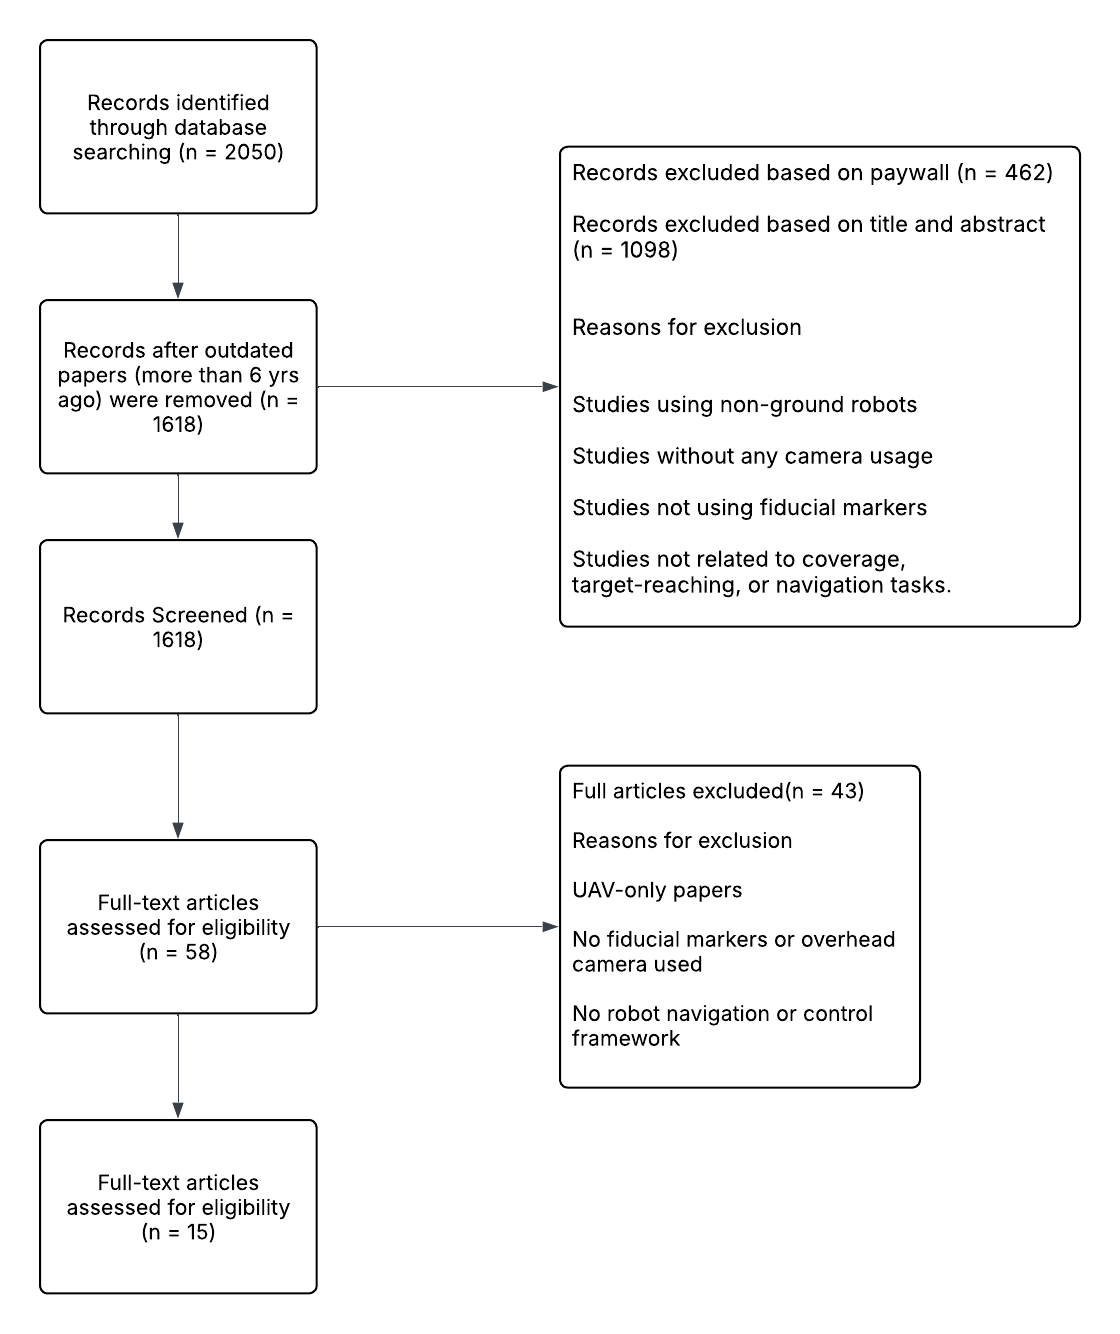
\includegraphics[width=0.7\linewidth]{chap2/images/figure_prisma.png}
    \caption{PRISMA 2020 Flowchart}
    \label{fig:figure_prisma}
\end{figure}

\section{Autonomous Navigation and Sensor Technologies}
Autonomous navigation fundamentally relies on a mobile robot’s ability to perceive its environment and determine its position relative to the environment. While autonomous navigation is a well established field, the hardware requirements for reliable performance remain a significant barrier for academic and low cost applications. In our review of literature on autonomous navigation, we found out that modern autonomous navigation relies on a heterogeneous sensor suite. Some of the most widely adopted technologies range from the classic RGB-D cameras , to innovations like event based sensors \citep{Gatesichapakorn2019ROSLidarRGBD, RodriguezMartinez2025VisionNavigationReview}. Recent multi-sensor approaches such as the work of \cite{Dai2023MultiSensorDocking}, who integrated LiDAR, YOLO-based AprilTag detection, and depth cues for autonomous docking, demonstrate how heterogeneous sensor fusion significantly improves docking precision and reliability in cluttered indoor environments. In this subchapter, we evaluate the advantages and disadvantages of each sensor technology.


\subsection{Monocular and Multicamera RGB Systems}
Monocular RGB cameras remain one of the most widely used sensing modalities in autonomous navigation due to their low cost, size, and ease of integration. Recent work demonstrates that deep learning greatly improves the capability of monocular systems, enabling better perception even without clear depth sensors. Research has shown that convolutional and transformer-based networks can infer scene geometry, obstacle layout, and traversability directly from RGB images 
\citep{Sleaman2022MonocularDNNNavigation}. Additional monocular systems, such as the neural-network-driven visual servoing framework by \cite{Jokic2019NNVisualServoing}, show how wide-FOV fisheye lenses combined with CNN-based controllers can enhance robustness even when depth cues are limited. Similarly, \cite{Ho2020PoseVisualServoing} demonstrated that pose-based visual servoing enhanced with lightweight deep-learning binarization improves tracking accuracy in resource-limited mobile robot platforms. These methods reduce hardware complexity while maintaining acceptable localization performance for indoor and structured environments.
Despite these advantages, monocular cameras suffer from an inherent depth ambiguity that can limit reliability in dynamic or cluttered spaces. Studies on monocular systems trained with deep reinforcement learning highlight that navigation performance largely depends on the variety of training environments \citep{Yokoyama2020DRLMonocularNavigation}. To help solve the depth limitation, recent research combines multiple deep learning modules and depth prediction to create better feature representations for navigation, as shown by \cite{Machkour2022MonocularNavigationMultipleDL}. These hybrid pipelines increase robustness but require more computational resources than classical monocular methods.

\subsection{RGB-D Cameras}
While Monocular and multi-camera RGB systems provide useful visual data for navigation, their lack of direct depth information restricts their robustness, especially in tasks requiring reliable 3D localization or obstacle avoidance. RGB-D cameras solve this problem by combining regular RGB images with depth information, producing a richer representation that simplifies tasks such as pose estimation, mapping, and collision detection. According to \cite{Civera2017RGBDOdometrySLAM}, RGB-D sensors are good alternatives to traditional range sensors like LiDAR because they are often cheap, compact, and require low-power, yet still provide both color and depth data that support 3D scene reconstruction. RGB-D sensing also appears in navigation pipelines such as the omnidirectional manufacturing-oriented robot proposed by \cite{Patruno2020VisionBasedOmniIndoor}, where combined RGB-D perception enables reliable autonomous movement in industrial indoor environments.

Many state-of-the-art approaches combine RGB-D data with odometry / SLAM pipelines to exploit this richer input. For instance, \cite{Gatesichapakorn2019ROSLidarRGBD} demonstrated a practical indoor navigation system using fused inputs from a 2D LiDAR and an RGB-D camera. This hybrid setup allowed a real mobile robot to navigate without a precomputed map. On the other hand, recent work such as \cite{Kostusiak2023EnhancingVOWithDepth} shows how modern deep-learning techniques can further improve performance: by refining noisy or incomplete depth maps (common with low-cost Kinect-like sensors), the study achieved more reliable indoor visual odometry under budget-friendly constraints.

\subsection{LiDAR and Camera-LiDAR Hybrids}
Recent studies highlight that combining LiDAR with cameras significantly improves autonomous navigation systems. According to \cite{Kolar2020DataFusionSurvey}, combining data from LiDAR and cameras lead to more accurate and robust mapping and localization, than just relying on either modality alone. There are studies that support this view, for example, \cite{DeSilva2018LidarWideAngleFusion}, designed a framework that  combined the use of LiDAR and wide-angle camera images and it resulted in significantly improved free-space detection performance. Hybrid LiDAR-vision architectures further align with the findings of \cite{Liu2022RobustLocalizationVisionCNN}, who showed that fusing CNN-based visual relocalization with progressive LiDAR scan-matching significantly enhances robustness under viewpoint changes and degraded visual conditions. However, these papers also highlight the limitation of the LiDAR-camera fusion which requires precise calibration and consistent environmental conditions that make real-time deployment more computationally demanding.

\subsection{Event-Based Cameras}
Event-based cameras output streams of “events” rather than fixed video frames, because of this, they offer compelling advantages for robotics and SLAM. According to \cite{Tenzin2024EventCamerasVSLAMSurvey}, event cameras deliver high temporal resolution, low latency, reduced power consumption and data bandwidth compared to traditional frame-based cameras. Additionally, the hardware architecture of this type of camera can efficiently handle the asynchronous event streams which enable low-power SLAM and perception on embedded robotic systems.

\subsection{Infrared and Thermal Imaging Sensors}
Infrared and thermal imaging sensors give strong advantages for autonomous robots especially in visually degraded and low-light environments. \cite{Papachristos_Mascarich_Alexis_2018b} showed that thermal imaging provides reliable localization for robots even in smoke, dust, or foggy conditions where performance of other cameras like RGB and LiDAR deteriorates. Similarly, recent work on Thermal SLAM by \cite{Salem2025ThermalSLAM}. demonstrates that temperature-based features can be used for object detection and tracking which improves localization regardless of lighting.

\subsection{Comparative Summary}
\begin{table}[H]
\centering
\setlength{\tabcolsep}{4pt} % reduce horizontal padding
\begin{tabular}{p{2.5cm} p{5cm} p{5cm}} % narrower columns
\hline
\textbf{Sensing Modality} & \textbf{Key Advantages} & \textbf{Major Limitations} \\
\hline
Monocular and Multicamera RGB &
\begin{itemize}
  \item Low cost, compact size, and ease of integration.
  \item Simplifies mapping and collision detection.
\end{itemize} &
\begin{itemize}
  \item Prone to noise or incomplete depth maps.
  \item Often limited to indoor ranges.
\end{itemize} \\
\hline
LiDAR \& Camera Hybrids &
\begin{itemize}
  \item Significantly improved free-space detection.
  \item More accurate and robust mapping than the single standalone of each part.
\end{itemize} &
\begin{itemize}
  \item Requires precise calibration.
  \item Computationally demanding for real-time deployment.
  \item Requires environmental consistency.
\end{itemize} \\
\hline
Event-Based Cameras &
\begin{itemize}
  \item High temporal resolution and low latency.
  \item Reduced power consumption and data bandwidth.
\end{itemize} &
\begin{itemize}
  \item Requires specific hardware architectures.
  \item Output is non-traditional (events) which requires specific processing.
\end{itemize} \\
\hline
Infrared \& Thermal Sensors &
\begin{itemize}
  \item Reliability in visually degraded conditions.
  \item Effective even in low-light, low visibility environments.
\end{itemize} &
\begin{itemize}
  \item Primarily focused on visually degraded conditions.
  \item Less feature rich for standard navigation.
\end{itemize} \\
\hline
\end{tabular}
\caption{Sensing modalities, advantages, and limitations.}
\label{tab:sensing_modalities}
\end{table}

As shown in Table 2.3, while LiDAR and Hybrid systems offer high accuracy, they suffer from high computational demands and calibration complexity. Conversely, Monocular RGB systems (Section 2.2.1) offer a balance of low cost and hardware simplicity. By leveraging Deep Learning—specifically the Neural Network architecture inherent in the DonkeyCar framework—this study aims to mitigate the 'depth ambiguity' limitation of monocular cameras by supplementing local vision with a global overhead supervisor (ArUco), thereby maintaining the low-resource benefits of RGB systems while improving navigation reliability.

\section{Computer Vision for Autonomous Robot Systems}
The computer vision systems in robotics systems serve as the eyes of the robot – providing vision that helps it recognize and understand its surroundings. Studies such as \cite{Alimovski2022VisionUrbanLocalization} also show that camera-only visual localization pipelines can remain effective even in complex, GPS-limited outdoor urban environments. Computer vision as defined by \cite{Vina2023CVInRoboticsIntegration}, is the technique where robotic systems use cameras and sensors to gather visual information.Then the information gathered is then processed by algorithms, which enable robots to perform complex tasks like assembly, quality control, and navigation. 

\subsection{LiDar and RTK-GPS and its Limitations}
LiDar and RTK-GPS (Real-Time Kinematic GPS), alone or in combination, are widely used to produce accurate mapping for vehicles \citep{DeMiguel2020ImprovedLidarProbabilistic, Thepsit2023LidarRTKGNSSINS}. However, there are several limitations that push for the implementation of alternative approaches for autonomous systems.

\subsubsection{Cost, Hardware, and Computational Requirements}
LiDar systems, as described by \cite{Whitaker2020GlobalLocalizationFiducialsIMU}, are often expensive and sizable for some applications. \cite{Lu2021LocalizationTechniquesReview} supports this idea in their study, concluding that LiDar is the most promising method for producing accurate, real-time localization among other approaches but suffers from the limitations of the system's computational ability, requiring more powerful CPU/GPU. This limitation poses a problem for smaller systems such as mobile robots where money, weight, and power consumption directly impact the navigation operations.

\subsubsection{GPS Signal Degradation and Denial}
RTK-GPS systems may suffer from extreme performance degradation or complete signal loss in a constrained environment such as urban canyons, underground or multi-level parking structures, tunnels, and indoor spaces \citep{Bhat2024MultiSourceGPSDenied, Fang2020MarkerValetParking, Jeon2021LaneAidedDeadReckoning}. Odometry errors accumulate fast without external correction, leading to inaccuracy in position estimates. \cite{Massa2020LidarGNSSDeniedRacing} resorted to alternative methods for a localization of self-driving racecars because GPS can be unreliable on racing tracks and in harsh environments. 

The limitations for LiDar and GPS collectively motivate the exploration of modern sensing modalities that can provide reliable localization in challenging scenarios where traditional systems struggle  \citep{Dreissig2023LiDARAdverseWeatherSurvey, Zhang2023AdverseWeatherPerceptionSurvey}. This  necessitates a need for developing alternative low‑cost computer‑vision approaches based on artificial fiducial markers that can provide reliable positioning without expensive sensors.

\subsection{Fiducial Marker Methods}
Fiducial markers are designed visual patterns which are machine or camera-detectable strategically placed within an environment to provide reliable localization mapping or pose estimation cues for autonomous systems. These visual markers serve as the landmarks that may offer multiple advantages over resource-intensive, natural or feature-based localization techniques. A broader mapping of marker-based navigation techniques is summarized in the systematic review by \cite{Alghamdi2025MobileRobotMarkersMapping}, which highlights the lightweight computational requirements, reliability, and adaptability of fiducial marker systems across diverse robotic domains.

In comparative studies of standard, custom, reflective, and infrared markers, fiducial markers generally offer high detection accuracy, robustness, and low computational cost, but their performance can still degrade under poor lighting conditions \cite{Alghamdi2025MobileRobotMarkersMapping}. Standard physical markers will include but not limited to, AR Tag \citep{Fiala2005ARTag}, AprilTag \citep{Olson2011AprilTag}, and AruCo markers \citep{GarridoJurado2014FiducialMarkers}.


\subsubsection{Operational Advantages}
When compared to localization methods like GPS RTK, the pragmatic advantages behind physical fiducial markers come from their ability to provide discrete, absolute position fixes that can correct accumulated drift in dead-reckoning systems \citep{Park2023FusionLocalizationAirplane, Xu2023VisualNavigationUAV}

Markers also facilitate the creation of persistent maps with known landmark positions. Unlike natural feature-based SLAM, which must continuously track and update potentially ambiguous environmental features, marker-based systems can rely on the stable, unambiguous identity and position of installed markers. This stability simplifies map maintenance and enables more predictable localization performance \citep{MunozSalinas2018SPMSLAM, Pfrommer2019TagSLAM, Wang_Zhang_Zhu_Hu_Deng_He_Kang_2023}. 

\subsubsection{Applications in Autonomous Systems}
Fiducial markers were leveraged to localization for vehicle parking in a GPS-denied setting like an underground parking lot for precise autonomous driving \citep{Fang2020MarkerValetParking}. Moreover, indoor autonomous drones use ceiling or wall mounted markers for positioning during warehouse inventory and structural examination tasks \citep{Nahangi2018UAVFiducialConstruction}. Marker systems have also been applied in assistive indoor navigation, such as the ARUCO-based pan-tilt camera system demonstrated by \cite{Adapa2019AutonomousMapping} for improving mobility support for blind and visually impaired users. Overhead or airborne localization frameworks similarly leverage markers, as seen in \cite{Xu2023VisualNavigationUAV}, who demonstrated a UAV-based visual navigation method using squared planar fiducials for orientation and path-following.

These applications share a common theme: they operate in environments where GPS is unavailable or unreliable, infrastructure modification is feasible, and cost-effective localization solutions are essential. Fiducial markers address these themes by providing a pragmatic middle ground between expensive LiDAR systems and drift-prone dead-reckoning approaches. The following section (2.5.3) details how these fiducial marker principles are realized in marker-based localization and mapping architectures, with a focus on ArUco-based systems.

\subsection{Marker-Based Localization, Mapping, and ArUco Systems}
Building on the general properties of fiducial markers outlined in Section 2.2.2, this section examines marker-based localization and mapping pipelines, emphasizing ArUco-based implementations in autonomous vehicles and robots.

\subsubsection{Detection and Pose Estimation}
Planar fiducial marker systems usually follow a structured pipeline that begins with image acquisition and proceeds through marker detection, corner localization, and pose estimation. In common implementations such as ArUco, candidate markers are extracted by thresholding and contour detection, followed by decoding of the internal binary pattern to recover marker identity and reject false positives \citep{Rosebrock2024ArucoPyImageSearch}. Once the four marker corners are localized in image coordinates and associated with a known marker size, the perspective‑n‑point (PnP) algorithm is used together with the camera calibration parameters to obtain the 6‑degrees-of-freedom (6-DoF) transformation between the marker frame and the camera frame \citep{Braun2022RobotAtFactoryLocalization, Fang2020MarkerValetParking}. This geometric formulation avoids any need for training data, and it provides an interpretable pose estimate that can be directly integrated into downstream localization and mapping pipelines.

\subsubsection{Robot and Camera Pose Tracking with ArUco}
Real-time implementations such as the UAV-mounted camera system in \cite{Waqas2022FiducialUAVSHM} confirm that marker-based pose tracking remains feasible even under dynamic motion, non-static camera poses, and rapid changes in scene geometry. Additionally, lightweight educational platforms, such as those in the Duckietown initiative by \cite{Krinkin2019DuckietownCalibration}, highlight how careful camera calibration and wheel-encoder integration support accurate pose estimation even on low-cost robotic systems.
When fiducial markers are deployed in the environment, each ArUco detection yields a relative pose measurement between the camera and the corresponding marker. Assuming a calibrated camera and known marker dimensions, these measurements can be expressed in metric units and transformed into a robot-centric or world-centric frame, enabling continuous tracking of the robot’s position and orientation as it moves through the environment \citep{Montecchio2022FiducialsUAV, Zhou2022UAVIndoorLocalization}. In practice, the system accumulates a time series of marker-based pose updates, which are combined with kinematic information such as wheel odometry to produce a smooth estimate of the robot trajectory in GPS‑denied settings.



\subsubsection{ArUco-based Planar Task-Space Localization}
Aside from providing global or relative pose measurements, planar fiducial configurations can be used to define local task spaces through homography estimation \citep{Braun2022RobotAtFactoryLocalization}. Numerous experimental systems have demonstrated the practicality of ArUco markers for autonomous vehicle and robot localization.

By placing multiple ArUco markers at the corners of a region of interest, \cite{Huang2022OptimizingMarkerPlacement} explored an optimized system that can compute a projective transformation between image coordinates and a planar world coordinate frame aligned with the physical surface. In addition, \cite{Rosner2025MultimodalIndoorDroneDataset} follows this idea for indoor drone tracking through markers on walls that define a room coordinate system (inside-out tracking). This demonstrates the efficacy of fiducial markers to provide planar task-space localization. \cite{Oh2025RegressionDockingAruco} applied this system for docking stations to achieve robust positioning with low-cost cameras and embedded processors. 

\subsubsection{Sensor Fusion Architectures}
In conventional autonomous systems, marker-based pose estimates are typically fused with proprioceptive sensors to compensate for intermittent visibility and measurement noise \citep{Kumar2023LocalizationSurveyAV}. Extended Kalman filters, error-state Kalman filters, and particle filters are widely used to combine discrete, absolute pose fixes from fiducial markers with continuous estimates derived from wheel encoders and inertial measurement units \citep{DeLaPuente2025VisionRangeAMCL, Ullah2020FilterLocalizationEvaluation}. Marker–odometry fusion has also been demonstrated effectively by \cite{Alam2023FiducialPFLocalization}, who showed that integrating AprilTag observations with particle filtering reduces drift and improves localization accuracy in indoor autonomous robots. In systems like these, the prediction step propagates the robot state forward using odometry or motion models, while the update step incorporates new marker observations when available, bounding drift and improving robustness when there is sensor noise and environmental disturbance.

\subsubsection{Marker-aided SLAM and Mapping}
In recent meta, mapping for autonomous robots are commonly carried out through LiDAR vision, which is costly and complex when it comes to maintenance \cite{Chen2025MapsAutonomousDrivingSurvey}. Traditional Marker-aided SLAM formulations incorporate fiducial markers as explicit landmarks in the map, rather than relying solely on natural point or line features \cite{Tourani2023MarkerBasedVisualSLAM}. In graph-based SLAM, markers are represented as nodes with fixed or estimated poses, and edges encode relative constraints between robot poses and marker observations; optimization of this graph improves both robot trajectories and marker maps \cite{MunozSalinas2018SPMSLAM}. This approach simplifies data association, because each marker carries a unique identifier, and supports persistent, globally consistent maps that can be reused across sessions, which is particularly advantageous in structured environments such as parking facilities and industrial halls.

Recent implementations reinforce the practical value of this paradigm. For example, \cite{Tolenov2024SelfLocalizationMapping} demonstrated a real-time camera-based SLAM pipeline capable of mapping unknown indoor environments without the use of LiDAR, showing that lightweight vision systems can be competitive when supported by robust tracking and optimization. Marker-enhanced localization pipelines also appear in aerial–ground hybrid systems such as \cite{Asif2020TetheredDroneLocalization}, where a tethered UAV and ground robot perform collaborative localization using deep neural networks supplemented by intermittent fiducial marker detections. These studies highlight how marker-aided SLAM can reduce cost, simplify data association through unique IDs, and enable persistent, reusable maps which are particularly beneficial in structured indoor environments.

\subsubsection{Gap Analysis for Marker-Based Detection and Localization}
While the literature establishes that marker-based sensor fusion and SLAM architectures (discussed in Sections 2.5.3.4 and 2.5.3.5) provide robust state estimation, they inherently introduce significant computational complexity and latency due to the iterative nature of Kalman filtering and graph optimization. Moreover, these traditional pipelines rely heavily on explicit state estimation. This requires the system to calculate the exact coordinates at every time step before making control decisions. This dependency introduces architectural complexity and computational overhead. Section 2.6 reviews recent advancements in deep learning for robot control, providing further justification for the shift away from traditional pose estimation toward end-to-end architectures.

\subsection{Modern Detection and Real-Time Systems}
Autonomous robots require vision-based localization pipelines that operate under strict real-time and resource constraints, often on embedded platforms such as single-board computers or low-power system-on-chip devices. The detection and pose estimation of fiducial markers must run at sufficient frame rates to support closed-loop control, while sharing computational resources with other perception and control modules. This has motivated a line of work focused on optimizing fiducial detection algorithms, memory usage, and numerical routines so that marker-based localization remains feasible on platforms with limited CPU, GPU, and power budgets \cite{Yulianto2025LightweightArucoDetection}.

\section{Deep Learning Approaches for Robot Control Strategies}
The integration of neural networks in autonomous systems have shifted the industry standard from hand-coded features, to data driven methodologies. In the context of autonomous mobile robot navigation, deep learning techniques have been increasingly used to process complex sensory data and generate navigational decisions. Upon reviewing literature, a survey from \cite{Xiao2022MLMotionPlanningSurvey} shows three deep learning paradigms for robot navigation; End-to-End Learning (E2E), Learning Subsystems, and Learning Components. Additionally, specific neural network architectures and training methodologies, referred to here as deep learning techniques, are employed across these paradigms to handle varied input modalities and control objectives. Recent marker- and vision-based navigation studies reinforce this trend. For instance, \cite{Liu2022RobustLocalizationVisionCNN} demonstrated that CNN-based relocalization can significantly improve pose recovery within a hybrid LiDAR-vision localization framework, showing how learned perception compensates for degraded geometric features. Deep neural controllers have also been applied to monocular systems, such as the visual servoing approach by \cite{Jokic2019NNVisualServoing}, which uses fisheye camera imagery to control a wheeled mobile robot. Similarly, \cite{Ho2020PoseVisualServoing} leveraged lightweight deep-learning binarization to enhance pose-based visual servoing for resource-constrained mobile robots. Hybrid aerial-ground systems such as \cite{Asif2020TetheredDroneLocalization} also illustrate how DNNs can infer relative positions between robots when fiducial marker signals are intermittent or partially occluded.
Together, these systems demonstrate that deep learning serves not only as a replacement for classical control but also as a complementary module for perception, relocalization, and decision-making within modern autonomous navigation architectures.

\subsection{Deep Learning Scopes}
The application of deep learning in autonomous mobile robot navigation is categorized by how much of the classical navigation stack (perception, localization, planning, and control) is replaced by neural networks. If the whole system is replaced with a neural network (E2E), if only subsystems of the navigation system are replaced (Learning Subsystems), or if only components (Learning Components).

End-to-End (E2E) Learning seeks to replace the classical navigation stack with a single deep neural network that maps raw inputs directly to control actions. This approach centralizes the process by integrating it into a single neural network process. \cite{Kim2018EndToEndNavigation}  demonstrated this by developing a deep learning model that processes RGB camera data to output steering in a single step. Similarly, \cite{Pierre2018EndToEndFollowing} applied E2E learning to robotic following behaviors, proving that a single network could learn complex tracking tasks without explicit object recognition modules.

Deep Learning Components, unlike E2E, involve replacing a single processing step within a module with a deep learning model. The most common application is in the perception module, where Convolutional Neural Networks (CNNs) replace manual feature extractors to perform object detection or semantic segmentation. For example, \cite{Redmon2016YOLO} introduced YOLO, a real-time object detection system that serves as a perception component, feeding bounding box coordinates to a classical costmap or planner. In this scope, the neural network does not make navigational decisions; it strictly provides structured information to a classical algorithm.

Deep Learning Subsystems replace an entire subprocess in the multi-step process of the autonomous robot navigation stack, while retaining the classical methods for the other parts. One such example is \cite{Mohanty2016DeepVO} DeepVO architecture proposal. The deep learning architecture replaces the classical visual odometry system with a Recurrent Convolutional Neural Network (RCNN). This subsystem takes raw video as input and outputs the robot's pose, directly replacing the localization module while leaving the planning and control modules untouched. A similar study from \cite{Faust_Ramirez_Fiser_Oslund_Francis_Davidson_Tapia_2017} proposed "PRM-RL," which replaces the local path planner subsystem with a Reinforcement Learning agent to handle dynamic obstacle avoidance, while still relying on a classical Probabilistic Roadmap (PRM) for global path planning. 

\subsection{Deep Learning Techniques}
Navigation systems often rely on specific neural network architectures and learning algorithms to process distinct data inputs, and generate control policies as outputs. Upon critical review on Literature, it is evident that the deep learning approaches of autonomous mobile robot navigation are driven by three architectural paradigms: Convolutional Neural Networks (CNNs), Recurrent Neural Networks (RNNs), and Vision Transformers (ViTs).

Convolutional Neural Networks are the most widely used approach in these systems. This can be attributed to the fact that CNNs are the best fit for the navigation pipeline. CNNs are best suited for processing spatial data such as camera images, depth maps, and lidar projections. The CNN can extract localized information from edges and textures to semantic level concepts, allowing robots to interpret complex environments reliably and efficiently \citep{LeCun2015DeepLearningNature}. This makes CNNs the best fit for perception tasks such as obstacle detection \citep{Eigen2014DepthSingleImage, Ronneberger2015UNet, Redmon2016YOLO}. This makes it the best fit for replacing the classical localization part of the navigation stack.

Recurrent neural networks (RNNs) are widely used in robot navigation due to their ability to model dependencies in sequential data such as robot odometry, velocity history, etc. Unlike CNNs, RNNs with LSTMs, and or GRUs are essential for predicting sequential robot trajectories, estimating future states, and generating smooth control commands \citep{Hochreiter1997LSTM, Cho2014RNNEncoderDecoder}. Recent Research incorporates RNNs with reinforcement learning or hybrid deep learning pipelines to better model robot-to-environment interactions. One example is the hybrid RNN architecture proposed by \cite{Radha2025HybridRNNNavigation} which demonstrates an improvement on optimization of path planning and collision avoidance by fusing temporal motion cues with spatial features extracted from CNNs Although studies also show that that RNN-based models significantly improve localization accuracy by including historical context, reducing hallucinations and localization drift, denoising movements, specifically in environments where GPS is not available \citep{Ichter2018LearningSamplingDistributions, Weng2019MotionForecastingRNN}.

Vision Transformers (ViTs) are a newer deep learning technique that is used in robot navigation, leveraging the breakthroughs in self-attention and the transformer model for vision based tasks. Unlike CNNs, which look at a group of fields at a time, CNNs process the data, its dependencies, and the semantics of each datapoint relative to each other. This helps robots interpret the whole environment, and consequently, plan out safe paths more effectively. \citep{Dosovitskiy2021ViT, Khan2022TransformersVisionSurvey}. Recent studies show that ViTs outperform CNNs in tasks requiring higher level semantic understanding or contextual awareness, such as large scale mapping, multiple map localization, contextual path planning, etc. \citep{Chen2021TransTrack}. Their ability to maintain performance under viewpoint changes, lighting variations, and occlusion makes them increasingly relevant for robust real-world navigation.

\section{Theoretical Framework}
This section outlines the mathematical models and fundamental theories utilized in the development of the autonomous navigation system. Specifically, it discusses the geometric principles of homography for localization, the algorithmic basis of fiducial marker detection, and the architecture of the deep learning approach used in the study.
\subsection{Projective Geometry and Planar Homography}
Since this study uses a single overhead camera to track a robot on a flat floor, the relationship between the camera’s image plane and the real world ground plane is defined by a planar homography. In computer vision, homography is defined as a fundamental projective transformation that maps points from one planar surface to another \cite{Hartley2003MultipleViewGeometry}. In our case, given an image point $p = (u, v, 1)^{t}$ and a corresponding point in the ground-plane coordinate system $p' = (x, y, 1)^{t}$, the planar homography relates them as 

\[
s
\begin{bmatrix}
x \\[2pt]
y \\[2pt]
1
\end{bmatrix}
=
H
\begin{bmatrix}
u \\[2pt]
v \\[2pt]
1
\end{bmatrix}
=
\begin{bmatrix}
h_{11} & h_{12} & h_{13} \\
h_{21} & h_{22} & h_{23} \\
h_{31} & h_{32} & h_{33}
\end{bmatrix}
\begin{bmatrix}
u \\[2pt]
v \\[2pt]
1
\end{bmatrix}
\]

where 
\begin{itemize}
    \item $s$ is an arbitrary scaling factor,
    \item $H$ is the $3\times3$ homography matrix,
    \item $(u,v)$ are the pixel coordinates of the marker,
    \item and $(x,y)$ are the metric coordinates on the floor.
\end{itemize}



To solve for the matrix $H$, at least four point correspondences are required. This study leverages the Direct Linear Transformation (DLT) algorithm to compute $H$ using calibrated anchors at the corners of the navigation arena, allowing for the real-time conversion of visual data into metric position estimates \citep{Szeliski2010ComputerVisionBook}.

\subsection{Neural Networks and Convolutional Neural Networks (CNNs)}
The control strategy that we proposed in this study is a CNN-based perception to actuation framework to provide end-to-end navigation controls. Unlike classical control methods like PID, which rely on a mathematical method for error correction, this study uses neural networks to approximate the non-linear relationship between the visual input and motor control, effectively emulating the thought process of a human driver. A neural network is a model that aims to imitate the functions of a human brain. It is made up of interconnected nodes (neurons) that are organized into different layers \citep{Goodfellow2016DeepLearning}. The fundamental operation involves transforming input data x into an input y through a series of weighted sums and non-linear activation functions:

\[
h_i = f_i\!\left(W_i h_{i-1} + b_i\right)
\]
where $h_i$ is the output of the $i$-th layer, $W_i$ and $b_i$
are the weight matrix and bias vector, and $f_i$ is the nonlinear
activation function.


This study employs a Convolutional Neural Network (CNN) architecture, which is highly effective for processing grid-like data such as images \citep{LeCun2015DeepLearningNature}. CNNs are characterized by three primary layer types that allow the system to learn spatial hierarchies automatically.

Convolutional Layers. These layers apply a set of kernels that slide over the input image, performing convolution operations to extract spatial features such as edges, textures, etc. The operation is defined as:
\[
(K * I)(i,j) =
\sum_{m}\sum_{n}
I(i - m,\, j - n)\, K(m,n)
\]

where $I$ is the input image, $K$ is the kernel, and $(i,j)$ are the
spatial coordinates.



Pooling Layers. These layers downsample the feature maps, reducing the dimensionality and the number of parameters. This helps make the features robust to slight shifts or distortions (e.g., Max-Pooling) while lowering the computational load.

Fully Connected Layers. Typically placed at the end of the CNN, these layers flatten the high-level features extracted by the convolutional and pooling layers and map them to the final output. In this study, the output corresponds to the continuous motor power commands (ie. left and right wheel velocities for Ackermann steering).

In the context of this research, CNN functions as an end-to-end policy network. It takes the homography-transformed overhead image, augmented with a digitally rendered coverage path, as input and regresses the optimal motor controls required to track that path. The network is trained using Behavioral Cloning, where the loss function (e.g., Mean Squared Error) minimizes the difference between the network's predicted actions and the human demonstrator's commands during the data collection phase. This approach allows the system to learn complex path-following behaviors directly from visual data, serving as a learned path follower component that bridges the gap between perception and control.

\subsection{Imitation Learning and Behavioral Cloning}
The study uses Imitation Learning as its deep learning approach. Imitation learning is the industry standard end-to-end approach based on our literature on Chapter 2. Imitation learning assumes access to expert demonstration. The goal is to learn a control policy  that mimics the behavior of the expert given specific state observations \citep{Osa2018ImitationLearningSurvey}.
More specifically, this study implements Behavioral Cloning, the simplest and most direct form of Imitation learning. Using this, the problem of learning a robot’s control policy is then reduced to a supervised learning task. The system collects a dataset $D$ consisting of $N$ pairs of observations and expert actions:
\[
D = \{(s_i, a_i)\}_{i=1}^{N}
\]
where $s_i$ represents the state observation (input) at time step $i$,
and $a_i$ represents the expert action (output) at time step $i$.



